\documentclass[autodetect-engine,dvipdfmx-if-dvi,ja=standard, 12pt]{bxjsarticle}

% 二段組にするとき
% \documentclass[twocolumn,autodetect-engine,dvipdfmx-if-dvi,ja=standard]{bxjsarticle}

\usepackage{graphicx}        %図を表示するのに必要
\usepackage{color}           %jpgなどを表示するのに必要
\usepackage{amsmath,amssymb} %数学記号を出すのに必要
\usepackage{setspace}
\usepackage{cases}
\usepackage{here}
\usepackage{fancyhdr}
\usepackage{ascmac}

\setlength{\textheight}{\paperheight}   % 紙面縦幅を本文領域にする(BOTTOM=-TOP)
\setlength{\topmargin}{3truemm}       % 上の余白を30mm(=1inch+4.6mm)に
\addtolength{\topmargin}{-\headheight}  %
\addtolength{\topmargin}{-\headsep}     % ヘッダの分だけ本文領域を移動させる
\addtolength{\textheight}{-50truemm}    % 下の余白も30mm(BOTTOM=-TOPだから+TOP+30mm)
% #################### Landscape Setting #######################
% # LEFT = 1inch + \hoffset + \oddsidemargin (\evensidemargin) #
% #      = 1inch + 0pt + 0pt                                   #
% # RIGHT = \paperwidth - LEFT - \textwidth                    #
% ##############################################################
\setlength{\textwidth}{\paperwidth}     % 紙面横幅を本文領域にする(RIGHT=-LEFT)
\setlength{\oddsidemargin}{-5.4truemm}  % 左の余白を25mm(=1inch-0.4mm)に
\setlength{\evensidemargin}{-5.4truemm} %
\addtolength{\textwidth}{-40truemm}     % 右の余白も25mm(RIGHT=-LEFT)

% 行頭の字下げをしない
\parindent = 0pt

% ヘッダとフッタの設定
\lhead{工業英語}
\chead{歩行者位置予測による運転抵抗を考慮した高度減速制御}
\rhead{5E 20番 佐藤凌雅}
\lfoot{}
\cfoot{-\thepage-} % ページ数
\rfoot{}

% 式の番号を(senction_num.num)のようにする
\makeatletter
\@addtoreset{equation}{section}
\def\theequation{\thesection.\arabic{equation}}
\makeatother

% 画像の貼り付けを簡単にする
\newcommand{\pic}[2]
{
  \begin{figure}[H]
    \begin{center}
      \includegraphics[scale=#2]{#1}
    \end{center}
  \end{figure}
}

% 単位の記述を簡単にする
\newcommand{\unit}[1]
{
  \, [\mathrm{#1}]
}
\begin{document}

\begin{abstract}
 本研究は,車両と歩行者との衝突を回避するための自動減速システムの実現を目的としている.提案システムは現在位置から歩行者の将来位置を予測し,衝突確率を検出することができる.さらに,駆動抵抗やモデリング誤差を補償することができるモデル予測制御を採用したコントローラも提案されている.提案した方法の有効性をシミュレーションと実験を通して検証した.
\end{abstract}

\maketitle
\pagestyle{fancy}

\section{前書き}
 近年,交通事故を減らす技術として自律型緊急ブレーキシステム(AEBS)が注目されている.しかしながら,現在の商用車のAEBSは,歩行者の現在位置に基づいて衝突の危険性を検出しており,歩行者の動きを考慮していないという問題がある.そのため,歩行者の動きに対応して,歩行者の将来の位置を予測し,それに応じて制動力を制御する必要がある.したがって,有限時間における車両の位置がシステムの指令値となるように,時間領域で車両を制御する必要がある.\\
 本論文での提案手法の概要は以下の通りである.まず,歩行者速度は,現在の歩行者の位置からカルマンフィルタによって推定される.将来の歩行者の予測位置は,一定期間の歩行者速度の値から予測される.衝突の可能性がある場合は,車両の予測位置と比較してMPCにより制動力の指令値を算出する. MPCは制約条件付きリアルタイム最適制御と呼ぶことができ,将来のシステム挙動を予測し,評価関数を最小化するように現在の入力値を決定する.MPCは開ループコントローラであるため,制御性能はモデル精度に大きく依存し,外乱の感度が高いという欠点がある.そこで,制御性能を向上させるために制動力のフィードバックループを導入し,外乱である駆動抵抗の推定量を提案システムに含める.さらに,駆動抵抗を補償して制動力を制御することで,外乱感度を低下させながらシステムの追従性を向上させることができる.\\

\section{モデリング}
\subsection{車体モデル}
 モデルを単純化するために直線運動のみを考慮した車両の車体モデルを図1に示す.\\
\begin{figure}[H]
    \centering
    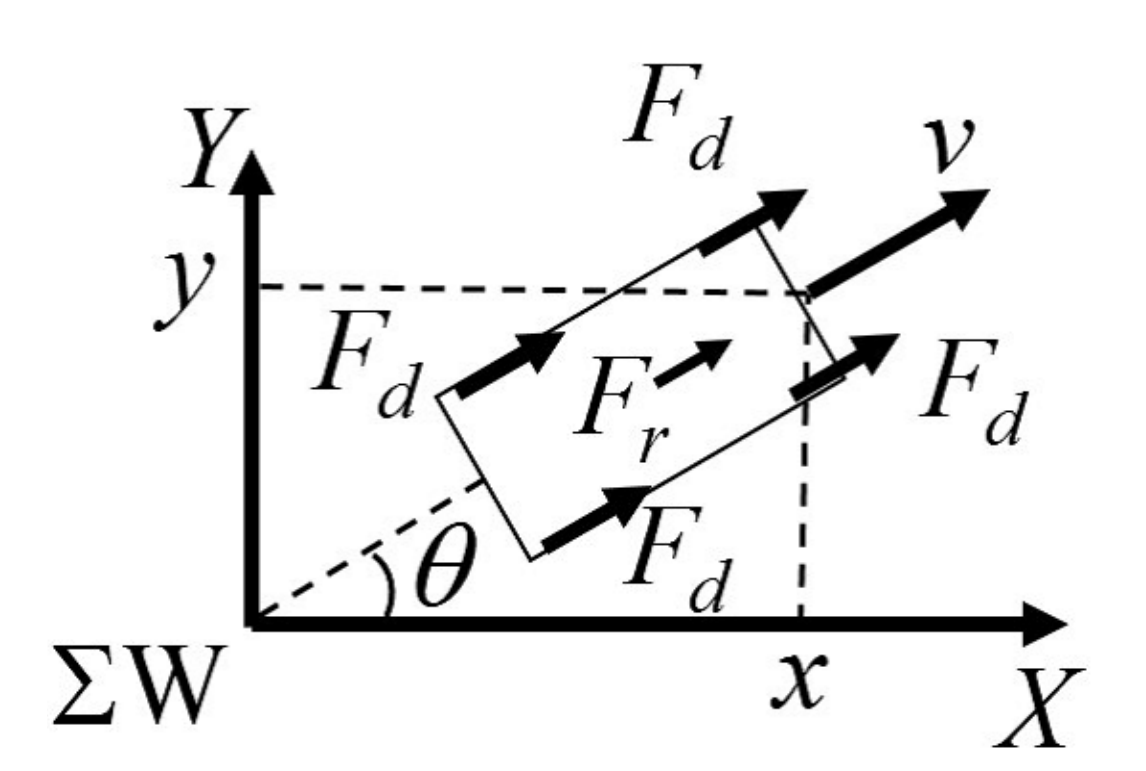
\includegraphics[height=3.5cm]{./fig/fig1.png}
    \caption{車両の車体モデル}
\end{figure}
 車両の車体の運動学とダイナミクスは次のとおり.\\
\begin{flalign}
    \dot{x} &= v\cos(\theta)\\
    \dot{y} &= v\sin(\theta)\\
    M\dot{v} &= nF_d+F_r
\end{flalign}

 ここで $x$ と $y$ は車両の位置である. $v$,$\theta$,$M$,$n$,$F_d$,$F_r$ は,それぞれ車速,車両角度,車両質量,制御輪数,駆動力,駆動抵抗である.$\Sigma$ はワールド座標系を表す.\\

\subsection{ホイールモデル}
\begin{flalign}
    J\dot{\omega} &= T_m - r_m F_d\\
    F_d &= \mu(\lambda)\frac{Mg}{n}\\
    \lambda &= \frac{v-r_\omega\omega}{\mbox{max}(v,r_\omega\omega)}
\end{flalign}
ホイールモデルのダイナミクスを示す.
ここで,$J$,$T_m$,$\omega$,$r_w$,$\lambda$,および$\mu$は,それぞれモーターの慣性,モーターまたはブレーキ装置によって生成されるトルク,車輪角速度,車輪半径,スリップ率,および摩擦係数を表す. $\mu$はスリップ率$\lambda$の関数である.

\section{制御システム設計}
\subsection{衝突検出}
 歩行者と車両の衝突を検出するために,最初にカルマンフィルターを使用して歩行者の速度を推定する.その後,有限時間における歩行者の位置が歩行者の速度から予測される.一定期間の歩行者の速度は2次正規分布に従うと想定される.これにより,確率密度関数が一定の場合,等確率楕円が作成される.これらを踏まえ,車両と歩行者が衝突する可能性があるかどうかは,以下の式を計算することで確認できる.
\begin{flalign}
    D &= \frac{(a+b)^2}{(c\sigma_u(iT_s+\tau)+R_h)^2} + \frac{(-a+b)^2}{(c\sigma_u(iT_s+\tau)+R_h)^2} \\
    a &= (\hat{x}_1[k+i|k] - \mu_x(iT_s + \tau) - x_h) \cos(\alpha)\\
    b &= (\hat{x}_2[k+i|k] - \mu_y(iT_s + \tau) - y_h) \sin(\alpha)\\
    \sigma_u^2 &= \frac{\sigma_x^2 + \sigma_y^2 + \sqrt{(\sigma_x^2 - \sigma_y^2) + 4\sigma_{xy}^2}}{2}\\
    \sigma_v^2 &= \frac{\sigma_x^2 + \sigma_y^2 - \sqrt{(\sigma_x^2 - \sigma_y^2) + 4\sigma_{xy}^2}}{2}\\
    \alpha &= \arctan \frac{\sigma_u^2 - \sigma_x^2}{\sigma_{xy}}
\end{flalign}
 $\mu_x$と$\mu_y$は平均値,$\alpha$は等確率楕円の角度を示す.
 $R_h$と$\tau$は,それぞれ歩行者の安全ゾーンの半径と計算のむだ時間を示している. $x_h$と$y_h$は歩行者の現在位置,$\sigma_x$、 $\sigma_y$は歩行者の速度の標準偏差,$\sigma_{xy}$は共分散である.μxとμyは一定期間内の歩行者の速度の平均を表す. $D$が1未満の場合,車両は歩行者の予測位置にあるため,衝突を避けるために減速する必要がある.
 $i_c$は,式(3.1)の$D\leq1$を満たす最小の$i$である.車両の現在位置により近い解が衝突回避の制限停止位置として採用され,$icTs$の停止司令点は制限位置から一定の距離にある位置となる.図2に,衝突検出のプロセスの概要を示す.
\begin{figure}[]
    \centering
    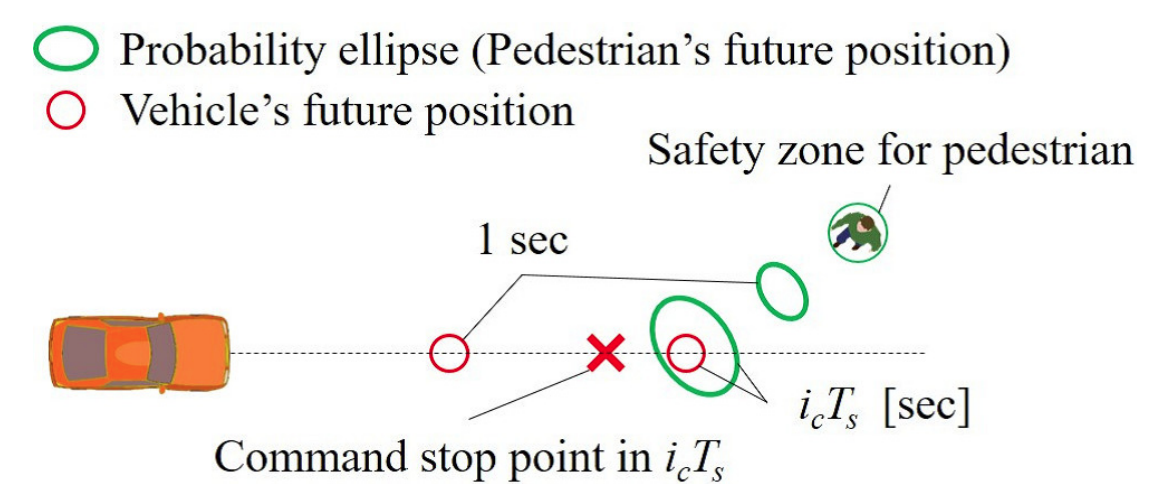
\includegraphics[height=3cm]{./fig/fig3.png}
    \caption{衝突検知の概要}
\end{figure}

\subsection{ブレーキコントロールシステム}
 モデル予測制御(MPC)は,車両を減速してicTsの停止位置で停止するために使用される. MPCは,入力を最適化すると同時に,いくつかの制約を使用して各時点で将来の応答を予測する制御方法である.
「コマンドの停止点を超える実行は行わない」,「入力の変化がチューニングパラメーターより小さくする」,「タイヤの力を摩擦円理論で決定される最大制動力よりも小さくする」といった制約の下,最適な入力変化$\Delta u [k|k]$が計算される.
計算された$\Delta u [k|k]$を用いて,各車輪の最適な制動力は次のように決定される.
\begin{flalign}
    F_d^{\mbox{cmd}} &= u[k-1]+\Delta u [k|k]
\end{flalign}

 ところでMPCはモデリングエラーを補正するためにフィードバックループが必要な開ループコントローラーである. したがって,MPCの内部でタイヤ力のフィードバックループを構築することが推奨されている.これを踏まえて,ブレーキ装置によって生成される基準トルクは次のように決定される.
\begin{flalign}
    T_m^{ref} &= \frac{K_i}{s}(F_d^{\mbox{cmd}} - \hat{F}_d)
\end{flalign}
 ここで,$K_i$および$\hat{F}_d$はそれぞれ,積分ゲイン,および駆動力オブザーバー(DFOB)によるタイヤ力の推定値を示す.

\subsection{オブザーバー設計}
 タイヤの力を推定するために,駆動力オブザーバー(DFOB)が使用される. DFOBは,外乱トルクを正確に推定できる外乱オブザーバー(DOB)に基づいていて,次のように定式化される.
\begin{flalign}
    \hat{F}_d &= \frac{1}{r_\omega}(\frac{g_{\mbox{cut}}}{s + g_{\mbox{cut}}}(T_m^{\mbox{ref}} + g_{\mbox{cut}} J\omega) - g_{\mbox{cut}} J\omega)
\end{flalign}
 ここで,$g_{\mbox{cut}}$はローパスフィルター(LPF)のカットオフ周波数を示す.
 最後に,ブレーキシステム全体を図3に示す.
\begin{figure}[H]
    \centering
    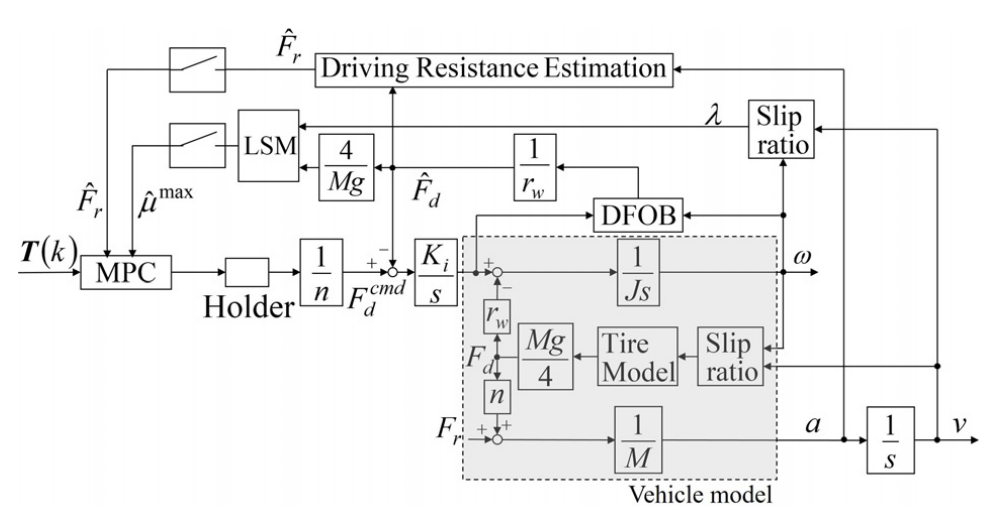
\includegraphics[height=4cm]{./fig/fig6.png}
    \caption{ブレーキシステムの全体}
\end{figure}

\section{シミュレーション}
\subsection{シミュレーション環境}
 提案手法の有効性を検証するために,シミュレーションを実施した. シナリオは,歩行者が横から出て,車両の前に到達すると停止するというものである.シミュレーションは,地面が乾いたダウンヒルと湿った平らな道路の2種類の道路環境で実行した.
\subsection{シミュレーション結果}
 シミュレーション1では,システムは良好に機能し,車両は運転抵抗を補償することで歩行者の前方に停止した.なお, 走行抵抗補正がない場合,車両は歩行者の前で停止できなかった.
 シミュレーション2のでは,路面が濡れていても最大摩擦係数を推定することにより,車両は歩行者の前方を停止した.なお,最大摩擦係数を推定しない場合,制動力が摩擦円理論の制限を超え,タイヤがスリップした.
 以上のことから,走行抵抗を考慮することの有効性が確認された.

\section{実験}
 提案された方法の有効性を確保するために実験を行った. 実験ではZMP Inc.が作成した1:10スケールの車両モデルであるRoboCar 1/10を使用した.この車両モデルには速度コントローラーが搭載されており,車両システムの入力は速度のみである. そのため,MPCから取得した速度値を入力に使用し,駆動力フィードバックの代わりに車両速度フィードバックを実装した.実験手順は次のとおり.
\begin{enumerate}
    \item PCで仮想歩行者の位置を生成
    \item PCが情報を車両に送信
    \item 車両は歩行者の位置を受け取り,制御を実行
  \end{enumerate}

 実験結果を図4,5に示す.図4は,車両と歩行者の位置を示している. 車両は歩行者の前の指令停止地点近くで停止した. このことから提案した方法が衝突回避システムとして十分機能することを示している. 図5からは走行抵抗推定値が定常値に収束していることがわかる.
 また,補償なしのブレーキシステムの場合ブレーキ力の変動が確認された. これはMPCが外乱と車両の状態を正確に予測できなかったためである. 以上より提案手法の有効性は実験により確認された.

\begin{figure}[H]
    \centering
    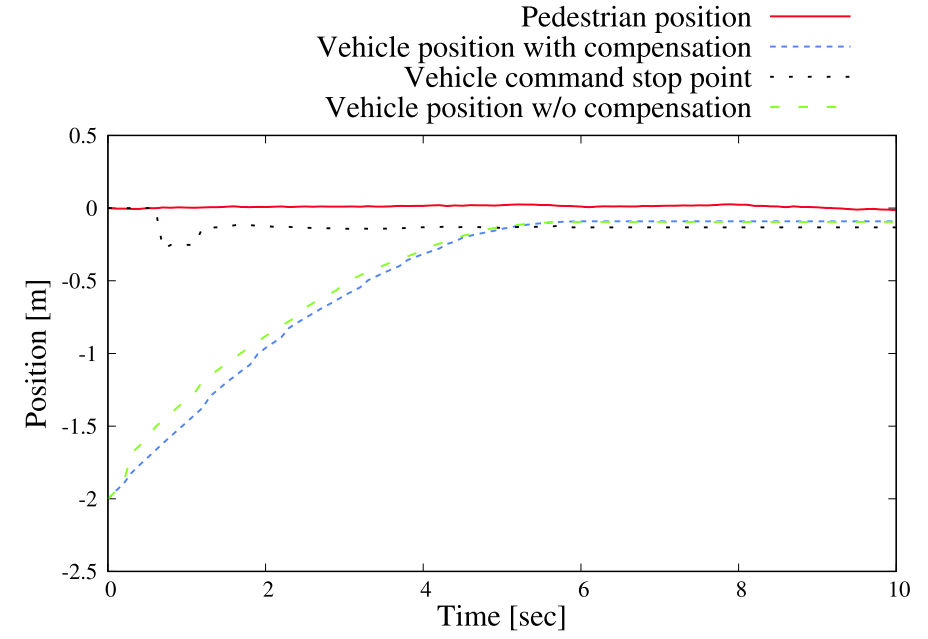
\includegraphics[height=4cm]{./fig/fig17.png}
    \caption{車両位置の実験結果}
  \end{figure}

\begin{figure}[H]
    \centering
    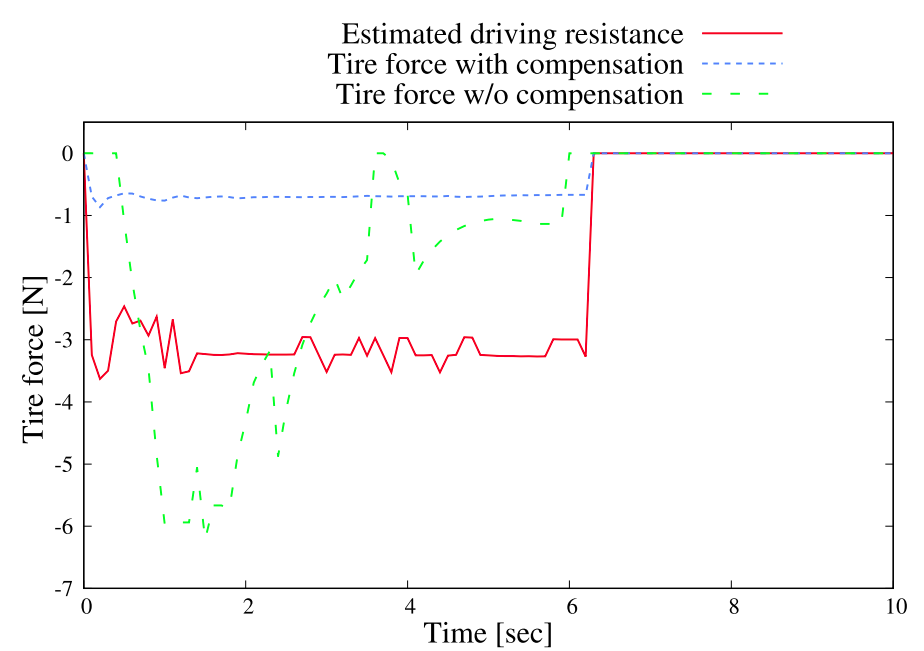
\includegraphics[height=4cm]{./fig/fig18.png}
    \caption{タイヤ力の実験結果}
  \end{figure}

\section{結論}
 本稿の目的は,歩行者との衝突を回避するために,自動減速システムを実現することである.提案システムは,現在の位置から歩行者の将来の位置を予測し,衝突確率を検出することが可能である.また,走行抵抗とモデル化誤差を補償することができるMPCとコントローラを,この論文で提案されている.
 まず,歩行者の速度は,カルマンフィルターにより,現在の歩行者の位置から推定される.将来の歩行者の予想位置は,歩行者の速度から予測され,制動力の指令値は,MPCによって計算される.ここでは,MPCは外乱とパラメータ誤差の影響を強く受けるため,制御性能を向上させるために,制動力のフィードバックループが提案されている.さらに,提案されたシステムには,走行抵抗の推定量が含まれている.これにより,歩行者の将来の位置を予測し,衝突の危険性を検出することが可能である.さらに,駆動抵抗を補償し,制動力を制御することにより,外乱感度を低減しながらシステムの追従性を向上させることができる.
 提案手法の有効性は,シミュレーションと実験により検証されている.このシステムを活用して,事故の数を減らすことが期待される.

\end{document}
